\documentclass[a4paper,14pt]{extreport} % формат документа

\usepackage{amsmath}
\usepackage{cmap} % поиск в ПДФ
\usepackage[T2A]{fontenc} % кодировка
\usepackage[utf8]{inputenc} % кодировка исходного текста
\usepackage[english,russian]{babel} % локализация и переносы
\usepackage[left = 2cm, right = 1cm, top = 2cm, bottom = 2 cm]{geometry} % поля
\usepackage{listings}
\usepackage{graphicx} % для вставки рисунков
\usepackage{amsmath}
\usepackage{float}
\usepackage{multirow}
\graphicspath{{pictures/}}
\usepackage{amsfonts}
\DeclareGraphicsExtensions{.pdf,.png,.jpg}
\newcommand{\anonsection}[1]{\section*{#1}\addcontentsline{toc}{section}{#1}}

\renewcommand{\thesection}{\arabic{section}}

\lstset{ %
	language=Matlab,                % Язык программирования 
	numbers=left,                   % С какой стороны нумеровать          
	frame=single,                    % Добавить рамку
	escapebegin=\begin{russian}\commentfont,
    escapeend=\end{russian},
    basicstyle=\small,
    literate={Ö}{{\"O}}1
    {Ä}{{\"A}}1
    {Ü}{{\"U}}1
    {ß}{{\ss}}1
    {ü}{{\"u}}1
    {ä}{{\"a}}1
    {ö}{{\"o}}1
    {~}{{\textasciitilde}}1
    {а}{{\selectfont\char224}}1
    {б}{{\selectfont\char225}}1
    {в}{{\selectfont\char226}}1
    {г}{{\selectfont\char227}}1
    {д}{{\selectfont\char228}}1
    {е}{{\selectfont\char229}}1
    {ё}{{\"e}}1
    {ж}{{\selectfont\char230}}1
    {з}{{\selectfont\char231}}1
    {и}{{\selectfont\char232}}1
    {й}{{\selectfont\char233}}1
    {к}{{\selectfont\char234}}1
    {л}{{\selectfont\char235}}1
    {м}{{\selectfont\char236}}1
    {н}{{\selectfont\char237}}1
    {о}{{\selectfont\char238}}1
    {п}{{\selectfont\char239}}1
    {р}{{\selectfont\char240}}1
    {с}{{\selectfont\char241}}1
    {т}{{\selectfont\char242}}1
    {у}{{\selectfont\char243}}1
    {ф}{{\selectfont\char244}}1
    {х}{{\selectfont\char245}}1
    {ц}{{\selectfont\char246}}1
    {ч}{{\selectfont\char247}}1
    {ш}{{\selectfont\char248}}1
    {щ}{{\selectfont\char249}}1
    {ъ}{{\selectfont\char250}}1
    {ы}{{\selectfont\char251}}1
    {ь}{{\selectfont\char252}}1
    {э}{{\selectfont\char253}}1
    {ю}{{\selectfont\char254}}1
    {я}{{\selectfont\char255}}1
    {А}{{\selectfont\char192}}1
    {Б}{{\selectfont\char193}}1
    {В}{{\selectfont\char194}}1
    {Г}{{\selectfont\char195}}1
    {Д}{{\selectfont\char196}}1
    {Е}{{\selectfont\char197}}1
    {Ё}{{\"E}}1
    {Ж}{{\selectfont\char198}}1
    {З}{{\selectfont\char199}}1
    {И}{{\selectfont\char200}}1
    {Й}{{\selectfont\char201}}1
    {К}{{\selectfont\char202}}1
    {Л}{{\selectfont\char203}}1
    {М}{{\selectfont\char204}}1
    {Н}{{\selectfont\char205}}1
    {О}{{\selectfont\char206}}1
    {П}{{\selectfont\char207}}1
    {Р}{{\selectfont\char208}}1
    {С}{{\selectfont\char209}}1
    {Т}{{\selectfont\char210}}1
    {У}{{\selectfont\char211}}1
    {Ф}{{\selectfont\char212}}1
    {Х}{{\selectfont\char213}}1
    {Ц}{{\selectfont\char214}}1
    {Ч}{{\selectfont\char215}}1
    {Ш}{{\selectfont\char216}}1
    {Щ}{{\selectfont\char217}}1
    {Ъ}{{\selectfont\char218}}1
    {Ы}{{\selectfont\char219}}1
    {Ь}{{\selectfont\char220}}1
    {Э}{{\selectfont\char221}}1
    {Ю}{{\selectfont\char222}}1
    {Я}{{\selectfont\char223}}1
    {і}{{\selectfont\char105}}1
    {ї}{{\selectfont\char168}}1
    {є}{{\selectfont\char185}}1
    {ґ}{{\selectfont\char160}}1
    {І}{{\selectfont\char73}}1
    {Ї}{{\selectfont\char136}}1
    {Є}{{\selectfont\char153}}1
    {Ґ}{{\selectfont\char128}}1
}

\begin{document}
\begin{titlepage}

    \begin{table}[H]
        \centering
        \footnotesize
        \begin{tabular}{cc}
            \multirow{8}{*}{
\includegraphics[scale=0.35]{bmstu.jpg}}
            & \\
            & \\
            & \textbf{Министерство науки и высшего образования Российской Федерации} \\
            & \textbf{Федеральное государственное бюджетное образовательное учреждение} \\
            & \textbf{высшего образования} \\
            & \textbf{<<Московский государственный технический} \\
            & \textbf{университет имени Н.Э. Баумана>>} \\
            & \textbf{(МГТУ им. Н.Э. Баумана)} \\
        \end{tabular}
    \end{table}

    \vspace{-2.5cm}

    \begin{flushleft}
        \rule[-1cm]{\textwidth}{3pt}
        \rule{\textwidth}{1pt}
    \end{flushleft}

    \begin{flushleft}
        \small
        ФАКУЛЬТЕТ
        \underline{<<Информатика и системы управления>>\ \ \ \ \ \ \ 
        \ \ \ \ \ \ \ \ \ \ \ \ \ \ \ \ \ \ \ \ \ \ \ \ \ \ \ \ \ \ \ 
    \ \ \ \ \ \ \ \ \ \ \ \ \ \ \ } \\
        КАФЕДРА
        \underline{<<Программное обеспечение ЭВМ и
        информационные технологии>>
        \ \ \ \ \ \ \ \ \ \ \ \ \ \ \ \ \ \ \ \ }
    \end{flushleft}

    \vspace{2cm}

    \begin{center}
        \textbf{Лабораторная работа № 2} \\
        \vspace{0.5cm}
    \end{center}

    \vspace{4cm}

    \begin{flushleft}
        \begin{tabular}{ll}
            \textbf{Дисциплина} & Математическая статистика.  \\
            \textbf{Тема} & Интервальные оценки.   \\
            \\
            \textbf{Студент} & Сиденко А.Г. \\
            \textbf{Группа} & ИУ7-63Б \\
            \textbf{Оценка (баллы)} & \\
            \textbf{Преподаватель} & Власов П.А.   \\
        \end{tabular}
    \end{flushleft}

    \vspace{4cm}

   \begin{center}
        Москва, 2020 г.
    \end{center}

\end{titlepage}

\section{Определение $\gamma$-доверительного интервала для значения параметра распределения случайной величины}

\hfill 

Дана случайная величина X, закон распределения которой известен с точностью до неизвестного параметра $\theta$. 

Интервальной оценкой с коэффициентом доверия $\gamma$ ($\gamma$-доверительной интервальной оценкой) параметра $\theta$ называют пару статистик $\underline{\theta}(\vec X), \overline{\theta}(\vec X)$ таких, что

$$P\{\underline{\theta}(\vec X)< \theta< \overline{\theta}(\vec X)\}=\gamma$$ 


Поскольку границы интервала являются случайными величинами, то для различных реализаций случайной выборки $\vec X$ статистики $\underline{\theta}(\vec X), \overline{\theta}(\vec X)$ могут принимать различные значения.

Доверительным интервалом с коэффициентом доверия $\gamma$ ($\gamma$-доверительным интервалом) называют интервал $(\underline{\theta}(\vec x), \overline{\theta}(\vec x))$, отвечающий выборочным значениям статистик $\underline{\theta}(\vec X), \overline{\theta}(\vec X)$. 

\section{Формулы для вычисления границ $\gamma$- доверительного интервала для математического ожидания и дисперсии нормальной случайной величины}

Формулы для вычисления границ $\gamma$- доверительного интервала для математического ожидания:

$$
\underline\mu(\vec X_n)=\overline X - \frac{S(\vec X)t_{\frac{1+\gamma}{2}}}{\sqrt{n}}
$$

$$
\overline\mu(\vec X_n)=\overline X + \frac{S(\vec X)t_{\frac{1+\gamma}{2}}}{\sqrt{n}}
$$

$\overline X$ -- точечная оценка математического ожидания

$S^2(\vec X)$ -- точечная оценка дисперсии

$n$ -- объем выборки

$\gamma$ -- уровень доверия

$t_{\frac{1+\gamma}{2}}$ -- квантили соответствующих уровней распределения Стьюдента с n - 1

Формулы для вычисления границ $\gamma$- доверительного интервала для дисперсии:

$$
\underline\sigma(\vec X_n)= \frac{(n-1)S^2(\vec X)}{h_{\frac{1+\gamma}{2}}}
$$

$$
\overline\sigma(\vec X_n)= \frac{(n-1)S^2(\vec X)}{h_{\frac{1-\gamma}{2}}}
$$

$S^2(\vec X)$ -- точечная оценка дисперсии

$n$ -- объем выборки

$\gamma$ -- уровень доверия

$h_{\frac{1+\gamma}{2}}$ -- квантили соответствующих уровней распределения хи-квадрат с n - 1

\section{Текст программы}

\hfill 

\begin{lstlisting}
function lab2()
    % Выборка объема n из генеральной совокупности Х
    X = [
 -7.50, -6.61, -7.85, -7.72, -8.96, -6.55, -7.82, -6.55, -6.87, -5.95, ...
 -5.05, -4.56, -6.14, -6.83, -6.33, -7.67, -4.65, -6.30, -8.01, -5.88, ...
 -5.38, -7.06, -6.85, -5.53, -7.83, -5.89, -7.57, -6.76, -6.02, -4.62, ...
 -8.55, -6.37, -7.52, -5.78, -6.12, -8.82, -5.14, -7.68, -6.14, -6.48, ...
 -7.14, -6.25, -7.32, -5.51, -6.97, -7.86, -7.04, -6.24, -6.41, -6.00, ...
 -7.46, -6.00, -6.06, -5.94, -5.39, -5.06, -6.91, -8.06, -7.24, -6.42, ...
 -8.73, -6.20, -7.35, -5.90, -5.02, -5.93, -7.56, -7.49, -6.26, -6.06, ...
 -7.35, -5.10, -6.52, -7.97, -5.71, -7.62, -7.33, -5.31, -6.21, -7.28, ...
 -7.99, -4.65, -7.07, -7.31, -7.72, -5.22, -7.00, -7.17, -6.64, -7.00, ...
 -6.12, -6.57, -6.07, -6.65, -7.60, -6.92, -6.78, -6.85, -7.90, -7.40, ...
 -5.32, -6.58, -6.71, -5.07, -5.80, -4.87, -5.90, -7.43, -7.03, -6.67, ...
 -7.72, -5.83, -7.49, -6.68, -6.71, -7.31, -7.83, -7.92, -5.97, -6.34, ...
 ];

    % Уровень доверия
    gamma = 0.9;
    % Объем выборки 
    n = length(X);
    % Точечная оценка матожидания
    mu = mean(X);
    % Точечная оценка дисперсии
    s2 = var(X);
    
    % Нижняя граница доверительного интервала для матожидания
    muLow = findMuLow(n, mu, s2, gamma);
    % Верхняя граница доверительного интервала для матожидания
    muHigh = findMuHigh(n, mu, s2, gamma);
    % Нижняя граница доверительного интервала для дисперсии
    s2Low = findS2Low(n, s2, gamma);
    % Верхняя граница доверительного интервала для дисперсии
    s2High = findS2High(n, s2, gamma);
    
    % Вывод полученных ранее значений
    fprintf('mu = %.3f\n', mu);
    fprintf('S2 = %.3f\n', s2);
    fprintf('muLow = %.3f\n', muLow);
    fprintf('muHigh = %.3f\n', muHigh);
    fprintf('s2Low = %.3f\n', s2Low);
    fprintf('s2High = %.3f\n', s2High);
    
    % Создание массивов точченых оценок
    muArray = zeros(1, n);
    s2Array = zeros(1, n);
    % Создание массивов границ доверительных интервалов
    muLowArray = zeros(1, n);
    muHighArray = zeros(1, n);
    s2LowArray = zeros(1, n);
    s2HighArray = zeros(1, n);
    
    % Цикл от 1 до n
    for i = 1 : n
        mu = mean(X(1:i));
        s2 = var(X(1:i));
        % Точечная оценка матожидания
        muArray(i) = mu;
        % Точечная оценка дисперсии
        s2Array(i) = s2;
        % Нижняя граница доверительного интервала для матожидания
        muLowArray(i) = findMuLow(i, mu, s2, gamma);
        % Верхняя граница доверительного интервала для матожидания
        muHighArray(i) = findMuHigh(i, mu, s2, gamma);
        % Нижняя граница доверительного интервала для дисперсии
        s2LowArray(i) = findS2Low(i, s2, gamma);
        % Верхняя граница доверительного интервала для дисперсии
        s2HighArray(i) = findS2High(i, s2, gamma);
    end
    
    % Построение графиков
    plot(1 : n, [(zeros(1, n) + mu)', muArray', muLowArray', muHighArray']);
    xlabel('n');
    ylabel('y');
    legend('$\hat \mu(\vec x_N)$', '$\hat \mu(\vec x_n)$', ...
        '$\underline{\mu}(\vec x_n)$', '$\overline{\mu}(\vec x_n)$', ...
        'Interpreter', 'latex', 'FontSize', 18);
    figure;
    plot(1 : n, [(zeros(1, n) + s2)', s2Array', s2LowArray', s2HighArray']);
    xlabel('n');
    ylabel('z');
    legend('$\hat S^2(\vec x_N)$', '$\hat S^2(\vec x_n)$', ...
        '$\underline{\sigma}^2(\vec x_n)$', '$\overline{\sigma}^2(\vec x_n)$', ...
        'Interpreter', 'latex', 'FontSize', 18);
end

% Функция поиска нижней границы доверительного интервала для матожидания
function muLow = findMuLow(n, mu, s2, gamma)
    muLow = mu - sqrt(s2) * tinv((1 + gamma) / 2, n - 1) / sqrt(n);
end

% Функция поиска верхней границы доверительного интервала для матожидания
function muHigh = findMuHigh(n, mu, s2, gamma)
    muHigh = mu + sqrt(s2) * tinv((1 + gamma) / 2, n - 1) / sqrt(n);
end

% Функция поиска нижней границы доверительного интервала для дисперсии
function s2Low = findS2Low(n, s2, gamma)
    s2Low = ((n - 1) * s2) / chi2inv((1 + gamma) / 2, n - 1);
end

% Функция поиска верхней границы доверительного интервала для дисперсии
function s2High = findS2High(n, s2, gamma)
    s2High = ((n - 1) * s2) / chi2inv((1 - gamma) / 2, n - 1);
end
\end{lstlisting}

\section{Результаты расчетов и графики для выборки из индивидуального варианта} 

\begin{enumerate}
\item Точечные оценки $\hat \mu (\vec x_N)$ и $ S^2 (\vec x_N)$ математического ожидания MX и дисперсии DX соответственно. 
\item Вычисление нижней и верхней границ $\underline \mu (\vec x_N)$, $\overline \mu (\vec x_N)$ для $\gamma$-доверительного интервала для математического ожидания DX. 
\item Вычисление нижней и верхней границ $\underline \sigma (\vec x_N)$, $\overline \sigma (\vec x_N)$ для $\gamma$-доверительного интервала для математического ожидания MX. 

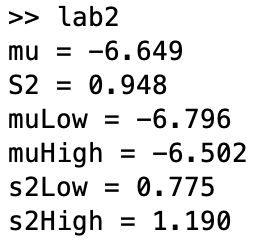
\includegraphics{values}

\item На координатной плоскости Oyn построить прямую $y=\hat \mu (\vec x_N)$, также графики функций $y=\hat \mu (\vec x_n), y= \underline \mu (\vec x_n), y =\overline \mu (\vec x_n)$ как функций объема n выборки, где n изменяется от 1 до N

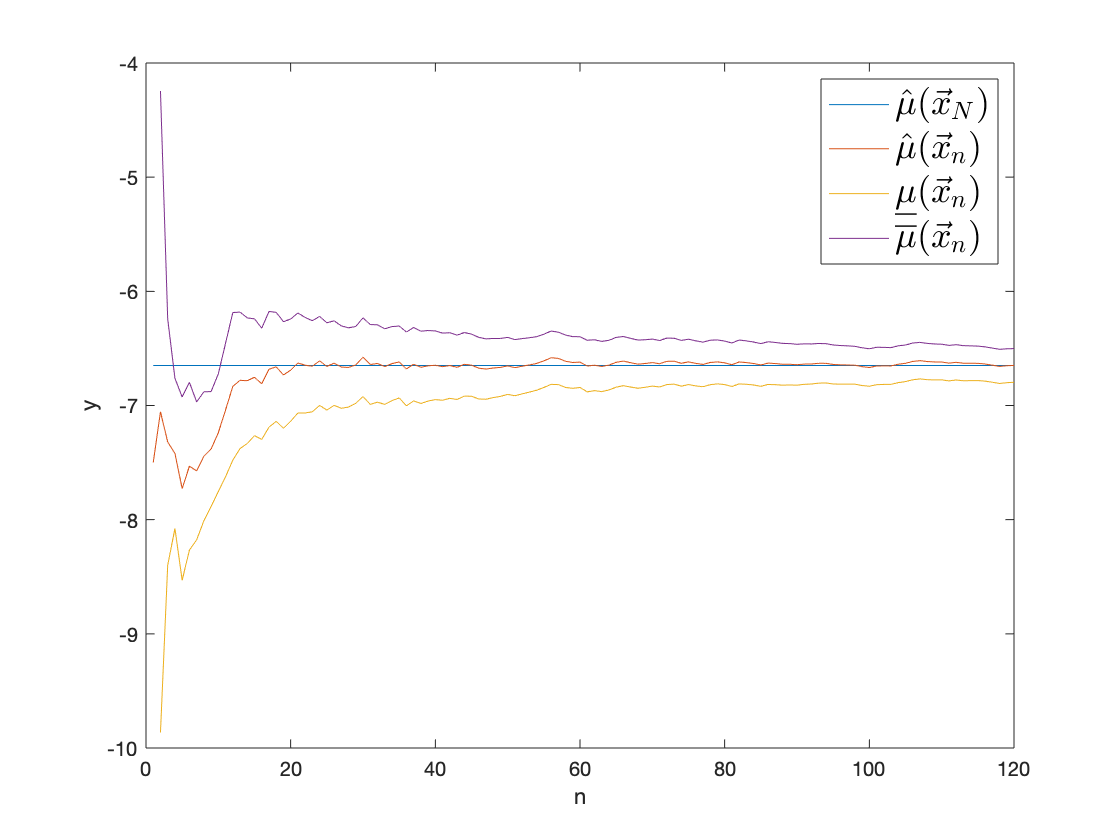
\includegraphics[scale=0.45]{graph1}

\newpage

\item На координатной плоскости Ozn построить прямую $z=\hat S^2 (\vec x_N)$, также графики функций $z= S^2 (\vec x_n), z= \underline \sigma^2 (\vec x_n), z =\overline \sigma^2 (\vec x_n)$ как функций объема n выборки, где n изменяется от 1 до N

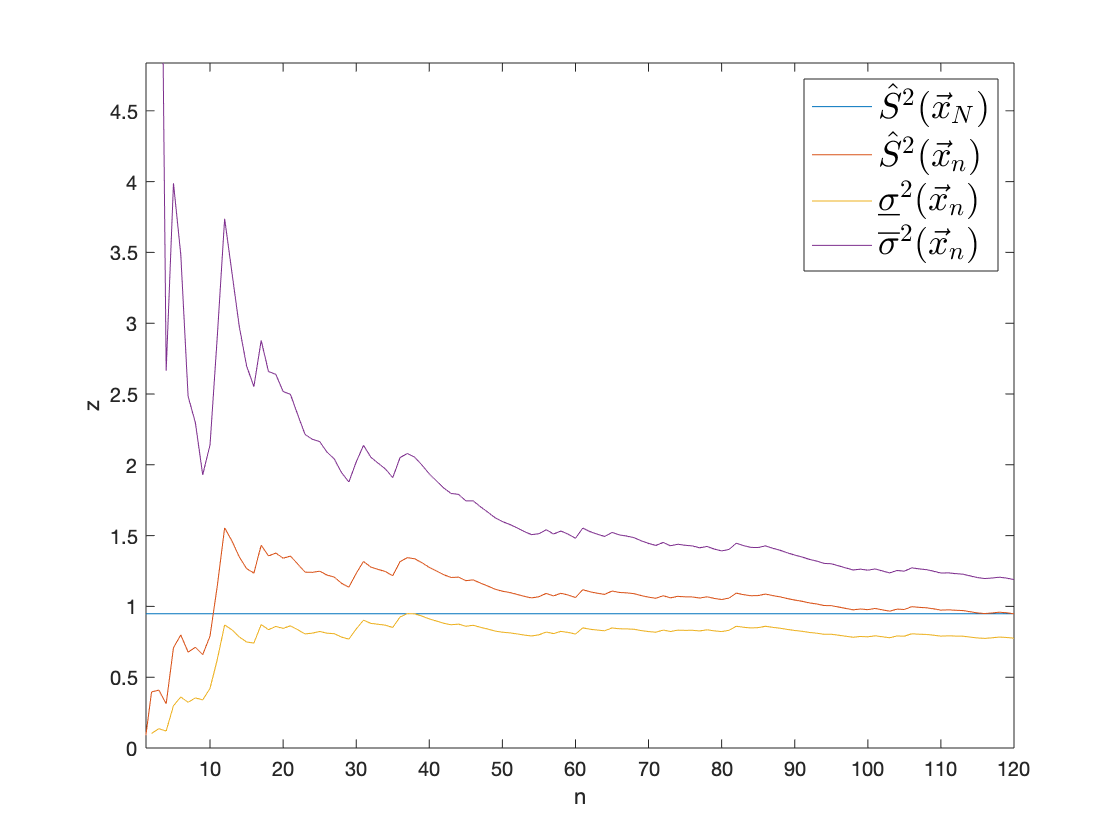
\includegraphics[scale=0.45]{graph2}

\end{enumerate}
\end{document}